\documentclass[11pt,a4paper]{report}
\usepackage[textwidth=37em,vmargin=30mm]{geometry}
\usepackage{calc,xunicode,amsmath,amssymb,paralist,enumitem,tabu,booktabs,datetime2,xeCJK,xeCJKfntef,listings}
\usepackage{tocloft,fancyhdr,tcolorbox,xcolor,graphicx,eso-pic,xltxtra,xelatexemoji}

\newcommand{\envyear}[0]{2025}
\newcommand{\envdatestr}[0]{2025-05-09}
\newcommand{\envfinaldir}[0]{webdb/2025/20250509/final}

\usepackage[hidelinks]{hyperref}
\hypersetup{
    colorlinks=false,
    pdfpagemode=FullScreen,
    pdftitle={Web Digest - \envdatestr}
}

\setlength{\cftbeforechapskip}{10pt}
\renewcommand{\cftchapfont}{\rmfamily\bfseries\large\raggedright}
\setlength{\cftbeforesecskip}{2pt}
\renewcommand{\cftsecfont}{\sffamily\small\raggedright}

\setdefaultleftmargin{2em}{2em}{1em}{1em}{1em}{1em}

\usepackage{xeCJK,xeCJKfntef}
\xeCJKsetup{PunctStyle=plain,RubberPunctSkip=false,CJKglue=\strut\hskip 0pt plus 0.1em minus 0.05em,CJKecglue=\strut\hskip 0.22em plus 0.2em}
\XeTeXlinebreaklocale "zh"
\XeTeXlinebreakskip = 0pt


\setmainfont{Brygada 1918}
\setromanfont{Brygada 1918}
\setsansfont{IBM Plex Sans}
\setmonofont{JetBrains Mono NL}
\setCJKmainfont{Noto Serif CJK SC}
\setCJKromanfont{Noto Serif CJK SC}
\setCJKsansfont{Noto Sans CJK SC}
\setCJKmonofont{Noto Sans CJK SC}

\setlength{\parindent}{0pt}
\setlength{\parskip}{8pt}
\linespread{1.15}

\lstset{
	basicstyle=\ttfamily\footnotesize,
	numbersep=5pt,
	backgroundcolor=\color{black!5},
	showspaces=false,
	showstringspaces=false,
	showtabs=false,
	tabsize=2,
	captionpos=b,
	breaklines=true,
	breakatwhitespace=true,
	breakautoindent=true,
	linewidth=\textwidth
}






\newcommand{\coverpic}[2]{
    % argv: itemurl, authorname
    Cover photo by #2~~(\href{#1}{#1})
}
\newcommand{\makeheader}[0]{
    \begin{titlepage}
        % \newgeometry{hmargin=15mm,tmargin=21mm,bmargin=12mm}
        \begin{center}
            
            \rmfamily\scshape
            \fontspec{BaskervilleF}
            \fontspec{Old Standard}
            \fontsize{59pt}{70pt}\selectfont
            WEB\hfill DIGEST
            
            \vfill
            % \vskip 30pt
            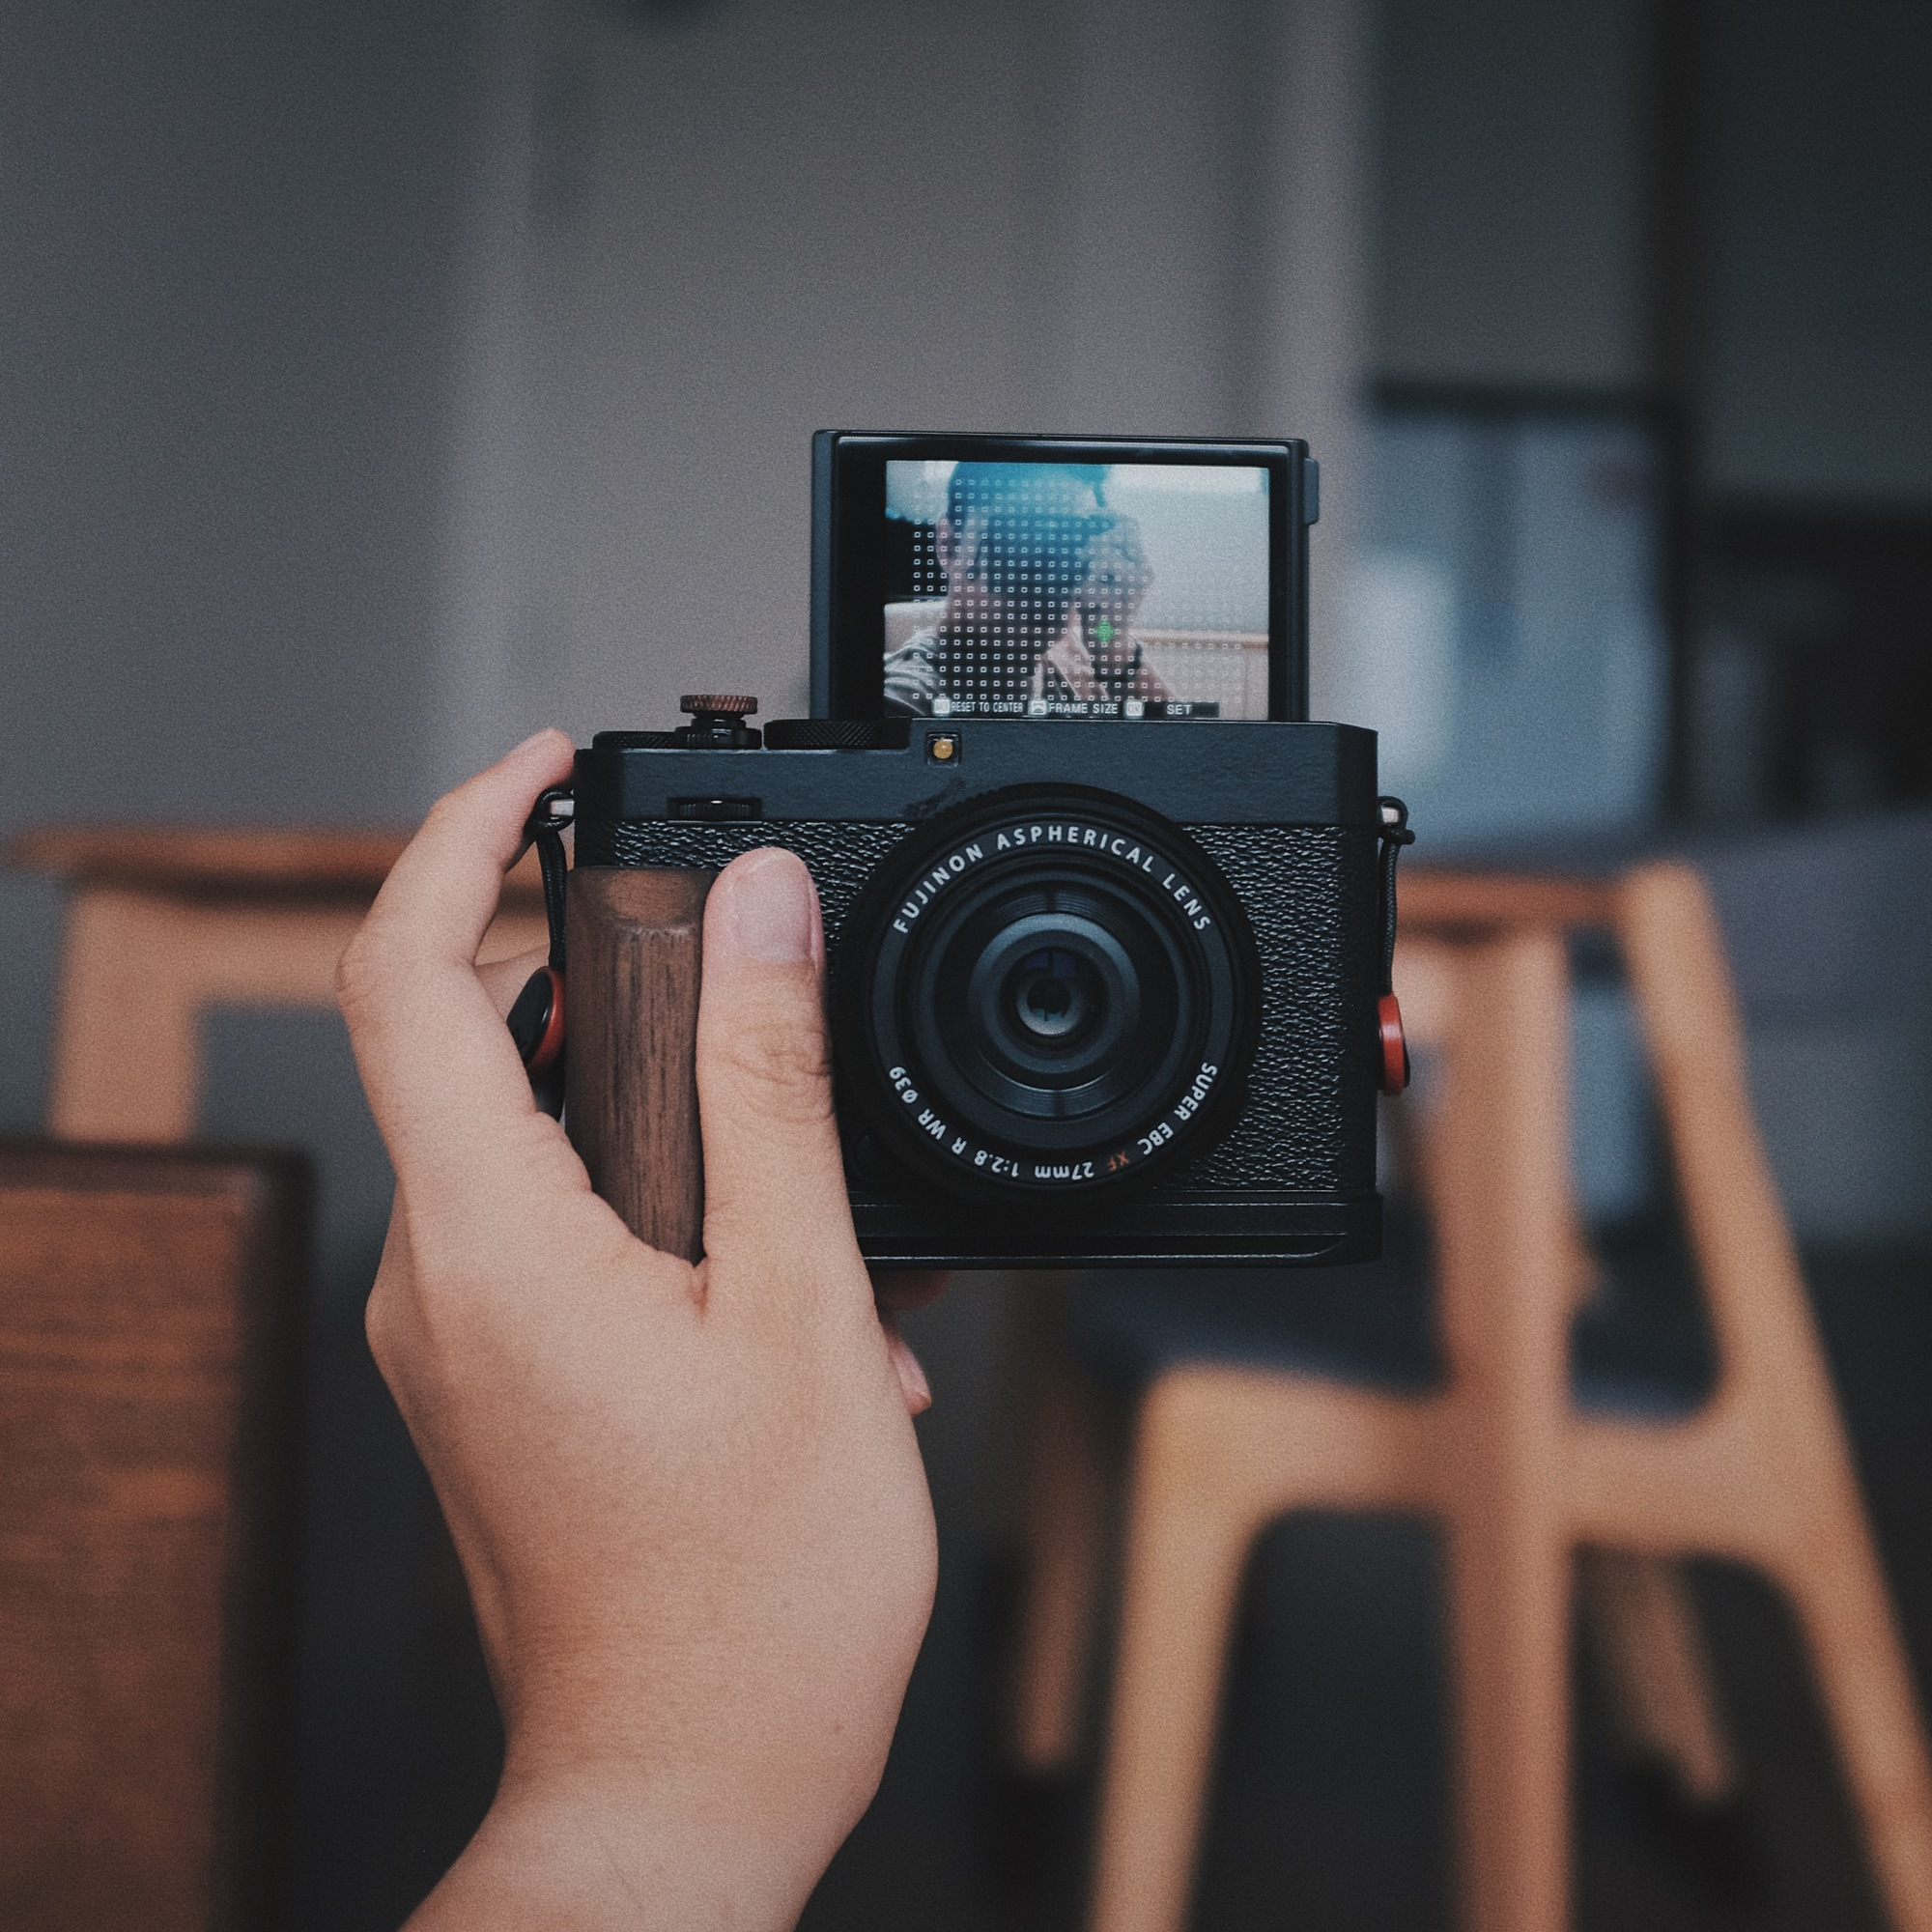
\includegraphics[width=\linewidth]{\envfinaldir/coverpic-prod.jpg}\par
            % \vskip 30pt
            \vfill

            \normalsize\rmfamily\scshape
            \copyright{} The Web Digest Project \hfill\large \envdatestr
        \end{center}
    \end{titlepage}
    % \restoregeometry
}
\newcommand{\simplehref}[1]{%
    \textcolor{blue!80!green}{\href{#1}{#1}}%
}
\renewcommand{\contentsname}{\center\Huge\sffamily\bfseries Contents\par\vskip 20pt}
\newcounter{ipartcounter}
\setcounter{ipartcounter}{0}
\newcommand{\ipart}[1]{
    % \vskip 20pt
    \clearpage
    \stepcounter{ipartcounter}
    \phantomsection
    \addcontentsline{toc}{chapter}{#1}
    % \begin{center}
    %     \Huge
    %     \sffamily\bfseries
    %     #1
    % \end{center}
    % \vskip 20pt plus 7pt
}
\newcounter{ichaptercounter}
\setcounter{ichaptercounter}{0}
\newcommand{\ichapter}[1]{
    % \vskip 20pt
    \clearpage
    \stepcounter{ichaptercounter}
    \phantomsection
    \addcontentsline{toc}{section}{\numberline{\arabic{ichaptercounter}}#1}
    \begin{center}
        \Huge
        \sffamily\bfseries
        #1
    \end{center}
    \vskip 20pt plus 7pt
}
\newcommand{\entrytitlefont}[1]{\subsection*{\raggedright\Large\sffamily\bfseries#1}}
\newcommand{\entryitemGeneric}[2]{
    % argv: title, url
    \parbox{\linewidth}{
        \entrytitlefont{#1}\par\vskip 5pt
        \footnotesize\ttfamily\mdseries
        \simplehref{#2}
    }\vskip 11pt plus 11pt minus 1pt
}
\newcommand{\entryitemGithub}[3]{
    % argv: title, url, desc
    \parbox{\linewidth}{
        \entrytitlefont{#1}\par\vskip 5pt
        \footnotesize\ttfamily\mdseries
        \simplehref{#2}\par\vskip 5pt
        \small\rmfamily\mdseries#3
    }\vskip 11pt plus 11pt minus 1pt
}
\newcommand{\entryitemAp}[3]{
    % argv: title, url, desc
    \parbox{\linewidth}{
        \entrytitlefont{#1}\par\vskip 5pt
        \footnotesize\ttfamily\mdseries
        \simplehref{#2}\par\vskip 5pt
        \small\rmfamily\mdseries#3
    }\vskip 11pt plus 11pt minus 1pt
}
\newcommand{\entryitemHackernews}[3]{
    % argv: title, hnurl, rawurl
    % \parbox{\linewidth}{
    %     \entrytitlefont{#1}\par\vskip 5pt
    %     \footnotesize\ttfamily\mdseries
    %     \simplehref{#3}\par
    %     \textcolor{black!50}{\href{#2}{#2}}
    % }\vskip 11pt plus 11pt minus 1pt
    \begin{minipage}{\linewidth}
            \entrytitlefont{#1}\par\vskip 5pt
            \footnotesize\ttfamily\mdseries
            \simplehref{#3}\par
            \textcolor{black!50}{\href{#2}{#2}}
    \end{minipage}\par\vskip 11pt plus 11pt minus 1pt
}







\begin{document}

\makeheader

\tableofcontents\clearpage




\ipart{Developers}
\ichapter{Hacker News}
\entryitemTwoLinks{From: Steve Jobs. "Great idea, thank you."}{https://news.ycombinator.com/item?id=43929724}{https://blog.hayman.net/2025/05/06/from-steve-jobs-great-idea.html}

\entryitemTwoLinks{Chicago native Cardinal Prevost elected pope, takes name Leo XIV}{https://news.ycombinator.com/item?id=43928742}{https://catholicreview.org/chicago-native-cardinal-prevost-elected-pope-takes-name-leo-xiv/}

\entryitemTwoLinks{Reservoir Sampling}{https://news.ycombinator.com/item?id=43928315}{https://samwho.dev/reservoir-sampling/}

\entryitemTwoLinks{Show HN: Using eBPF to see through encryption without a proxy}{https://news.ycombinator.com/item?id=43928118}{https://github.com/qpoint-io/qtap}

\entryitemTwoLinks{Void: Open-source Cursor alternative}{https://news.ycombinator.com/item?id=43927926}{https://github.com/voideditor/void}

\entryitemTwoLinks{Notes on rolling out Cursor and Claude Code}{https://news.ycombinator.com/item?id=43927914}{https://ghiculescu.substack.com/p/nobody-codes-here-anymore}

\entryitemTwoLinks{First American pope elected and will be known as Pope Leo XIV}{https://news.ycombinator.com/item?id=43927856}{https://www.cnn.com/world/live-news/new-pope-conclave-day-two-05-08-25}

\entryitemTwoLinks{High tariffs become 'real' with our first \$36K bill}{https://news.ycombinator.com/item?id=43927813}{https://blog.adafruit.com/2025/05/08/high-tariffs-become-real-with-our-first-36k-bill/}

\entryitemTwoLinks{Progress toward fusion energy gain as measured against the Lawson criteria}{https://news.ycombinator.com/item?id=43927337}{https://www.fusionenergybase.com/articles/continuing-progress-toward-fusion-energy-breakeven-and-gain-as-measured-against-the-lawson-criteria}

\entryitemTwoLinks{My new deadline: 20 years to give away virtually all my wealth}{https://news.ycombinator.com/item?id=43926165}{https://www.gatesnotes.com/home/home-page-topic/reader/n20-years-to-give-away-virtually-all-my-wealth}

\entryitemTwoLinks{Trump's NIH axed research grants even after a judge blocked the cuts}{https://news.ycombinator.com/item?id=43926149}{https://www.propublica.org/article/trump-nih-cuts-transgender-research-grants}

\entryitemTwoLinks{Google to back three new nuclear projects}{https://news.ycombinator.com/item?id=43925982}{https://www.esgtoday.com/google-to-back-three-new-advanced-nuclear-projects/}

\entryitemTwoLinks{Microservices are a tax your startup probably can't afford}{https://news.ycombinator.com/item?id=43925892}{https://nexo.sh/posts/microservices-for-startups/}

\entryitemTwoLinks{Ask HN: What are good high-information density UIs (screenshots, apps, sites)?}{https://news.ycombinator.com/item?id=43925732}{https://news.ycombinator.com/item?id=43925732}

\entryitemTwoLinks{Using NASA's SMAP satellite to detect L-band interference}{https://news.ycombinator.com/item?id=43924358}{https://radioandnukes.substack.com/p/how-dare-you-transmit-at-14-ghz}

\entryitemTwoLinks{Mycoria is an open and secure overlay network that connects all participants}{https://news.ycombinator.com/item?id=43923372}{https://mycoria.org/}

\entryitemTwoLinks{We have reached the "severed fingers and abductions" stage of crypto revolution}{https://news.ycombinator.com/item?id=43923187}{https://arstechnica.com/security/2025/05/we-have-reached-the-severed-fingers-and-abductions-stage-of-the-crypto-revolution/}

\entryitemTwoLinks{Ask HN: How much better are AI IDEs vs. copy pasting into chat apps?}{https://news.ycombinator.com/item?id=43922759}{https://news.ycombinator.com/item?id=43922759}

\entryitemTwoLinks{Show HN: US Routing – Python library for fast local routing in the US}{https://news.ycombinator.com/item?id=43921653}{https://github.com/ivanbelenky/us-routing}

\entryitemTwoLinks{Yggdrasil is an experimental compact routing scheme that is fully decentralised}{https://news.ycombinator.com/item?id=43921624}{https://yggdrasil-network.github.io/about.html}\ichapter{Phoronix}
\entryitemGeneric{\hskip 0pt{}Intel Begins Posting Linux Patches For Wildcat Lake}{https://www.phoronix.com/news/Intel-Wildcat-Lake-Linux-Begins}

\entryitemGeneric{\hskip 0pt{}Intel Link-Off Between Frames "LOBF" Submitted For Linux 6.16 Graphics Driver}{https://www.phoronix.com/news/Intel-LOBF-For-Linux-6.16}

\entryitemGeneric{\hskip 0pt{}Qualcomm Snapdragon X Elite Benchmarks On Ubuntu Linux vs. AMD vs. Intel}{https://www.phoronix.com/review/snapdragon-x-elite-linux-benchmarks}

\entryitemGeneric{\hskip 0pt{}Few Apple Silicon Device Tree Updates Submitted Ahead Of Linux 6.16}{https://www.phoronix.com/news/Apple-Silicon-DT-Linux-6.16}

\entryitemGeneric{\hskip 0pt{}OpenRazer 3.10.3 Brings Linux Driver Support For Razer's Naga V2 Pro \& Strider Chroma}{https://www.phoronix.com/news/OpenRazer-3.10.3}

\entryitemGeneric{\hskip 0pt{}Linux 6.16 Bringing A Fix For Old Intel Haswell Graphics}{https://www.phoronix.com/news/Linux-6.16-Intel-Haswell-iGPU}

\entryitemGeneric{\hskip 0pt{}DragonFlyBSD Sees Progress On UVC Webcam Support}{https://www.phoronix.com/news/DragonFlyBSD-UVC-Webcam-Sort-Of}

\entryitemGeneric{\hskip 0pt{}Mesa 25.2 Merges AMD Support For Setting Queue Priorities}{https://www.phoronix.com/news/Mesa-25.2-AMDGPU-Queue-Priority}

\entryitemGeneric{\hskip 0pt{}Python 3.14 Reaches Beta With New Tail-Call Interpreter For Better Performance}{https://www.phoronix.com/news/Python-3.14-Beta-1}\ichapter{Dribbble}
\entryitemGeneric{\hskip 0pt{}CTRL the Chaos // Dashboard}{https://dribbble.com/shots/25997365-CTRL-the-Chaos-Dashboard}

\entryitemGeneric{\hskip 0pt{}Modernizing the Website of a Shopify Email Customizer}{https://dribbble.com/shots/25993532-Modernizing-the-Website-of-a-Shopify-Email-Customizer}

\entryitemGeneric{\hskip 0pt{}Travel Startup Branding for Holidu: visual identity brand design}{https://dribbble.com/shots/25941954-Travel-Startup-Branding-for-Holidu-visual-identity-brand-design}

\entryitemGeneric{\hskip 0pt{}Western Union Logo Redesign Concept}{https://dribbble.com/shots/25991687-Western-Union-Logo-Redesign-Concept}

\entryitemGeneric{\hskip 0pt{}Luvi Wordmark Design}{https://dribbble.com/shots/25994954-Luvi-Wordmark-Design}

\entryitemGeneric{\hskip 0pt{}The Neovision Way}{https://dribbble.com/shots/25994705-The-Neovision-Way}

\entryitemGeneric{\hskip 0pt{}AI Security}{https://dribbble.com/shots/25987123-AI-Security}

\entryitemGeneric{\hskip 0pt{}Fiyah > Hot Sauces Line}{https://dribbble.com/shots/25989187-Fiyah-Hot-Sauces-Line}

\entryitemGeneric{\hskip 0pt{}Just a Hippo}{https://dribbble.com/shots/25988582-Just-a-Hippo}

\entryitemGeneric{\hskip 0pt{}Crypto Portfolio Tracker App}{https://dribbble.com/shots/25988631-Crypto-Portfolio-Tracker-App}

\entryitemGeneric{\hskip 0pt{}Unused Logo Concept for FinAi}{https://dribbble.com/shots/25989542-Unused-Logo-Concept-for-FinAi}

\entryitemGeneric{\hskip 0pt{}Houston Oaks}{https://dribbble.com/shots/25991694-Houston-Oaks}

\entryitemGeneric{\hskip 0pt{}Tees High™ Monogram}{https://dribbble.com/shots/25990424-Tees-High-Monogram}

\entryitemGeneric{\hskip 0pt{}Mobile App Work Session Tracker}{https://dribbble.com/shots/25975579-Mobile-App-Work-Session-Tracker}

\entryitemGeneric{\hskip 0pt{}Fellowship Church - Branding}{https://dribbble.com/shots/25990448-Fellowship-Church-Branding}

\entryitemGeneric{\hskip 0pt{}Quartz Wordmark Logo}{https://dribbble.com/shots/25985137-Quartz-Wordmark-Logo}

\entryitemGeneric{\hskip 0pt{}Fianance Landing Page}{https://dribbble.com/shots/25980595-Fianance-Landing-Page}

\entryitemGeneric{\hskip 0pt{}Envisioning the future}{https://dribbble.com/shots/25985271-Envisioning-the-future}

\entryitemGeneric{\hskip 0pt{}Heliara}{https://dribbble.com/shots/25983106-Heliara}

\entryitemGeneric{\hskip 0pt{}UI/UX Design for AURA — your personal AI assistant}{https://dribbble.com/shots/25982086-UI-UX-Design-for-AURA-your-personal-AI-assistant}

\entryitemGeneric{\hskip 0pt{}GOCCO Wordmark}{https://dribbble.com/shots/25984476-GOCCO-Wordmark}

\entryitemGeneric{\hskip 0pt{}Lume}{https://dribbble.com/shots/25978139-Lume}

\entryitemGeneric{\hskip 0pt{}Illustration}{https://dribbble.com/shots/25975830-Illustration}

\entryitemGeneric{\hskip 0pt{}Medical Landing Page Design}{https://dribbble.com/shots/25971117-Medical-Landing-Page-Design}


\ipart{Developers~~~~(zh-Hans)}
\ichapter{Solidot}
\entryitemGeneric{\hskip 0pt{}Gmail 停止支持 3DES 加密的传入 SMTP 连接}{https://www.solidot.org/story?sid=81239}

\entryitemGeneric{\hskip 0pt{}今天出生的人更可能遭遇极端气候事件}{https://www.solidot.org/story?sid=81238}

\entryitemGeneric{\hskip 0pt{}curl 项目遭遇 AI 生成的虚假漏洞报告攻击}{https://www.solidot.org/story?sid=81237}

\entryitemGeneric{\hskip 0pt{}特朗普政府计划修改拜登时代的 AI 芯片出口限制}{https://www.solidot.org/story?sid=81236}

\entryitemGeneric{\hskip 0pt{}人才评价机制僵化导致论文工厂屡铲不除}{https://www.solidot.org/story?sid=81235}

\entryitemGeneric{\hskip 0pt{}基因突变让部分人每天只需要睡 3 小时}{https://www.solidot.org/story?sid=81234}

\entryitemGeneric{\hskip 0pt{}欧盟制定吸引美国科学家的政策}{https://www.solidot.org/story?sid=81233}

\entryitemGeneric{\hskip 0pt{}因违反打包政策 openSUSE 移除 Deepin Desktop}{https://www.solidot.org/story?sid=81232}

\entryitemGeneric{\hskip 0pt{}绿地与新生儿的健康相关}{https://www.solidot.org/story?sid=81231}

\entryitemGeneric{\hskip 0pt{}《原神》向美国用户引入年龄验证}{https://www.solidot.org/story?sid=81230}

\entryitemGeneric{\hskip 0pt{}科学家研发出可结构重编程的磁性超材料}{https://www.solidot.org/story?sid=81229}

\entryitemGeneric{\hskip 0pt{}巴基斯坦恢复对 X 的访问}{https://www.solidot.org/story?sid=81228}

\entryitemGeneric{\hskip 0pt{}体罚对儿童具有完全负面影响}{https://www.solidot.org/story?sid=81227}

\entryitemGeneric{\hskip 0pt{}Reddit CEO 称员工太理想主义而没有努力工作}{https://www.solidot.org/story?sid=81226}

\entryitemGeneric{\hskip 0pt{}美国公司 CEO 离职率创下记录}{https://www.solidot.org/story?sid=81225}

\entryitemGeneric{\hskip 0pt{}Ubuntu 25.10 将默认使用 sudo-rs}{https://www.solidot.org/story?sid=81224}

\entryitemGeneric{\hskip 0pt{}微软对因绩效不佳而解雇的员工实施两年禁聘令}{https://www.solidot.org/story?sid=81223}

\entryitemGeneric{\hskip 0pt{}特朗普政府官员使用的修改版 Signal 暂停服务}{https://www.solidot.org/story?sid=81222}

\entryitemGeneric{\hskip 0pt{}Mr. Deepfakes 永久关闭}{https://www.solidot.org/story?sid=81221}

\entryitemGeneric{\hskip 0pt{}古代诗歌揭示江豚的历史分布}{https://www.solidot.org/story?sid=81220}\ichapter{V2EX}
\entryitemGeneric{\hskip 0pt{}[云计算] 大家帮我看看这个 traceroute 有没有问题?}{https://www.v2ex.com/t/1130558}

\entryitemGeneric{\hskip 0pt{}[问与答] Clash 怎么配置实现外网回家?}{https://www.v2ex.com/t/1130557}

\entryitemGeneric{\hskip 0pt{}[汽车] 小警示,一个办理 etc 的骗子}{https://www.v2ex.com/t/1130556}

\entryitemGeneric{\hskip 0pt{}[软件] 写了个 app 去监督自己代码进度}{https://www.v2ex.com/t/1130554}

\entryitemGeneric{\hskip 0pt{}[问与答] 如何用 edu 邮箱秒过 cursor 学生认证,成功白嫖一年会员。}{https://www.v2ex.com/t/1130553}

\entryitemGeneric{\hskip 0pt{}[云修电脑] 请大神帮忙看看是不是硬盘出问题了,}{https://www.v2ex.com/t/1130551}

\entryitemGeneric{\hskip 0pt{}[职场话题] 选外包还是死磕甲方}{https://www.v2ex.com/t/1130550}

\entryitemGeneric{\hskip 0pt{}[问与答] Windows 笔记本可以一键迁移资料吗}{https://www.v2ex.com/t/1130549}

\entryitemGeneric{\hskip 0pt{}[投资] 回应 v 友的质疑,黄金我没有卖....}{https://www.v2ex.com/t/1130548}

\entryitemGeneric{\hskip 0pt{}[分享创造] 搓了个究极轻量的文档系统}{https://www.v2ex.com/t/1130547}

\entryitemGeneric{\hskip 0pt{}[问与答] 各位大佬有无便宜稳定的 ai 视频生成 api 平台推荐}{https://www.v2ex.com/t/1130546}

\entryitemGeneric{\hskip 0pt{}[微软] 比尔·盖茨宣布将在未来 20 年内捐出几乎所有财富}{https://www.v2ex.com/t/1130544}

\entryitemGeneric{\hskip 0pt{}[NAS] 纯稳定、便利且长期家庭数据存储,不知道什么方案才合适了。}{https://www.v2ex.com/t/1130542}

\entryitemGeneric{\hskip 0pt{}[OpenAI] 为什么 OpenAI 要收购 Windsurf?}{https://www.v2ex.com/t/1130541}

\entryitemGeneric{\hskip 0pt{}[macOS] macOS 音量均衡软件推荐哪款?在任何 app 下播放出来的声音始终能一样,不用频繁调节各个音量大小。}{https://www.v2ex.com/t/1130540}

\entryitemGeneric{\hskip 0pt{}[分享创造] 分享下自己搞的一个 Markdown 文档批量工具 mdctl}{https://www.v2ex.com/t/1130539}

\entryitemGeneric{\hskip 0pt{}[前端开发] shadcn-vue 使用 Tips}{https://www.v2ex.com/t/1130538}

\entryitemGeneric{\hskip 0pt{}[分享发现] cursor 秒过新方法,需要 edu 邮箱}{https://www.v2ex.com/t/1130537}

\entryitemGeneric{\hskip 0pt{}[生活] 关于要不要提前还房贷,想听听大家想法呢}{https://www.v2ex.com/t/1130536}

\entryitemGeneric{\hskip 0pt{}[问与答] 为什么银行普遍不支持 Passkey?}{https://www.v2ex.com/t/1130535}

\entryitemGeneric{\hskip 0pt{}[酷工作] 广州外企 - Principal Data Framework Engineer - 50-80k}{https://www.v2ex.com/t/1130533}

\entryitemGeneric{\hskip 0pt{}[职场话题] 有人收到过大中厂 offer 么,求一个邮件}{https://www.v2ex.com/t/1130530}

\entryitemGeneric{\hskip 0pt{}[职场话题] 每天也没干什么高强度的事情, 6 点下班,但是就是困....}{https://www.v2ex.com/t/1130529}

\entryitemGeneric{\hskip 0pt{}[数据库] sqlite 需要彻底移除已删除的敏感字段,跑一下 VACUUM 就够物理删除了吗?}{https://www.v2ex.com/t/1130528}

\entryitemGeneric{\hskip 0pt{}[分享发现] Manus campus 放水了,有在列表内 edu 邮箱的可以直接注册}{https://www.v2ex.com/t/1130525}

\entryitemGeneric{\hskip 0pt{}[程序员] 想买个 win 的 小主机,日常办公用,大家有没有推荐的款项?}{https://www.v2ex.com/t/1130524}

\entryitemGeneric{\hskip 0pt{}[程序员] 最近遇到了 3 次非常难查的问题,很无助}{https://www.v2ex.com/t/1130523}

\entryitemGeneric{\hskip 0pt{}[Apple] 用惯了五年前 LG 的 42C1,再用 studio display,简直失望透顶, 1 万多的显示器居然显示不了黑}{https://www.v2ex.com/t/1130522}

\entryitemGeneric{\hskip 0pt{}[问与答] gmail 提示说一个月内把我的区域改成美国华盛顿,如果不同意可以提工单,大家遇到过这个情况吗,求指点,理由是更好的服务}{https://www.v2ex.com/t/1130521}

\entryitemGeneric{\hskip 0pt{}[问与答] 接了个单,想问一下有没有法律风险?}{https://www.v2ex.com/t/1130520}

\entryitemGeneric{\hskip 0pt{}[宽带症候群] 武汉电信自营营业厅 修改宽带账号 可以恢复真公网 ipv4 解除上传 5Mbps 限制}{https://www.v2ex.com/t/1130519}

\entryitemGeneric{\hskip 0pt{}[问与答] 想在昆明住一两个月,哪里体验最好呀?}{https://www.v2ex.com/t/1130518}

\entryitemGeneric{\hskip 0pt{}[酷工作] 现在 IOS 开发都是什么价位啊?}{https://www.v2ex.com/t/1130517}

\entryitemGeneric{\hskip 0pt{}[iOS] 双持 ios 和 android, app 同步怎么处理}{https://www.v2ex.com/t/1130516}

\entryitemGeneric{\hskip 0pt{}[DNS] 为什么用了阿里的 DOH 还会解析到江苏反诈? 用其他 DOH 就不会}{https://www.v2ex.com/t/1130515}

\entryitemGeneric{\hskip 0pt{}[分享创造] 做了个 llms.txt 生成器,据说对 SEO 有好处}{https://www.v2ex.com/t/1130514}

\entryitemGeneric{\hskip 0pt{}[问与答] 最近很少看到一个大厂技术公众号推技术方案的文章了}{https://www.v2ex.com/t/1130513}

\entryitemGeneric{\hskip 0pt{}[iOS] 感觉备忘录的检索速度没以前快了,是错觉吗?}{https://www.v2ex.com/t/1130511}

\entryitemGeneric{\hskip 0pt{}[问与答] 做下面一个服务号和小程序 大概需要多少成本}{https://www.v2ex.com/t/1130510}

\entryitemGeneric{\hskip 0pt{}[问与答] 新奇玩意,遇到支付相关的开发需求,可惜了解甚少啊,做个分享求助帖}{https://www.v2ex.com/t/1130508}

\entryitemGeneric{\hskip 0pt{}[奇思妙想] 完全不同意 Google 搜索会被 Gen AI 颠覆,相反,我觉得 Google 会受益于 LLM 技术。}{https://www.v2ex.com/t/1130506}

\entryitemGeneric{\hskip 0pt{}[问与答] 有蜗牛网盘的阿里云第三方平替吗,阿里云盘最近操作太恶心了}{https://www.v2ex.com/t/1130505}

\entryitemGeneric{\hskip 0pt{}[买买买] 乐歌电动升降桌推荐吗?}{https://www.v2ex.com/t/1130504}

\entryitemGeneric{\hskip 0pt{}[程序员] 开发在线 Playground 的实践}{https://www.v2ex.com/t/1130503}

\entryitemGeneric{\hskip 0pt{}[职场话题] [北京] 京东零售招人了,招前端,主要用 next.js, 有意者联系 v: d29pd29ya2luZw==,或者发简历到 bGludW8yMUBqZC5jb20=也可以,最近已经给俩 V2EX 好友发 offer 了,机会多多,快来}{https://www.v2ex.com/t/1130502}

\entryitemGeneric{\hskip 0pt{}[推广] HornetPay 虚拟 visa 卡, 1 刀开卡,长期有效}{https://www.v2ex.com/t/1130500}

\entryitemGeneric{\hskip 0pt{}[问与答] 中国联通升级``二次号码焕新''服务,一键解决历史遗留绑定账号}{https://www.v2ex.com/t/1130499}

\entryitemGeneric{\hskip 0pt{}[职场话题] 运维工作 6 年后,感觉面试基本不问我技术了}{https://www.v2ex.com/t/1130497}

\entryitemGeneric{\hskip 0pt{}[旅行] 5 月底打算去川西玩 5 天,是自驾还是报团呢?}{https://www.v2ex.com/t/1130496}

\entryitemGeneric{\hskip 0pt{}[Spotify] 谁能救救我的每周推荐}{https://www.v2ex.com/t/1130495}


\ipart{Generic News}
\ichapter{联合早报}
\entryitemWithDescription{黎康:魔都的B面}{https://www.zaobao.com/news/china/story20250426-6241474}{``确实这几年上海的城市公共建设很好,但你有没有去看过一些老旧小区的环境?小区里电线横飞,绿化基本毫无规划;进入楼道,你会感觉回到20年前\ldots\ldots'' 上一篇``早点------沪上闲语''发表后,收到一封读者来信。这位上海市民告诉我,在装点城市门面的郁金香背后,如果走进上海的老旧小区,会看到这座城市的另一面……}

\entryitemWithDescription{新闻人间:从``不懂球的胖子''到改革推手——刘国梁}{https://www.zaobao.com/news/china/story20250426-6238850}{中国乒乓球协会星期三(4月23日)突然宣布,刘国梁主动辞去主席一职。这一消息迅速引发体坛热议,有球迷为他的离开感到惋惜,也有体育评论员开始审视他在任期内的功与过。 刘国梁自2018年起担任乒协主席,如今在第二任期尚未结束之际中途请辞,外界难免有诸多猜测。星期三当天,他以主席身份在乒协会议上作最后一次发言时,几度哽咽,甚至当场落泪。 他在记者会上透露,早在去年巴黎奥运会结束后,便已向上级表达了去意……}

\entryitemWithDescription{中国据报考虑暂停加征部分美国产品125\%关税}{https://www.zaobao.com/news/china/story20250425-6245926}{中国政府据报考虑暂停对部分美国进口产品加征125\%的关税,受访学者认为此举主要考虑中国企业的生存需要,与中美是否开启贸易谈判无关。 据彭博社引述知情人士报道,中国政府正考虑取消对美国的医疗设备,以及乙烷等工业化学品加征的报复性关税。中国是全球最大的塑料制造国,但部分工厂依赖从美国进口的乙烷。中国医院也需要美国生产的磁共振成像和超声仪器等医疗设备。 知情人士称,飞机租赁也可能豁免关税……}

\entryitemWithDescription{中国美国商会白皮书:五分之一美企不再视中国为优先投资地}{https://www.zaobao.com/news/china/story20250425-6245113}{中国美国商会的调查显示,五分之一的在华美国企业不再将中国列为优先的投资目的地。 该商会星期五(4月25日)发布由100余名中国美国商会会员企业代表共同撰写的2025年《美国企业在中国白皮书》。 白皮书指出,中美两国关系日益紧张,已连续五年成为在华美资企业面临的首要商业挑战,超过了合规风险和来自中国企业的竞争压力……}

\entryitemWithDescription{中国发布生态调查报告 称菲律宾捕捞现场发现人为弃置物}{https://www.zaobao.com/news/china/story20250425-6244616}{(北京讯)中国多家自然生态机构星期五(4月25日)联合公布一份调查报告,评估铁线礁、牛轭礁珊瑚礁的生态系统状况,称菲律宾所谓``中国在铁线礁倾倒珊瑚碎屑等言论''毫无科学和事实依据。 中国自然资源部微信公号分别发表了这份题为《铁线礁、牛轭礁珊瑚礁生态系统调查报告》的中英文版本,参与编制的机构包括中国自然资源部南海发展研究院、南海生态中心等……}

\entryitemWithDescription{香港公共场所明年起设更多禁烟区 违例罚款提高一倍}{https://www.zaobao.com/news/china/story20250425-6245064}{为了进一步降低吸烟率,香港特区政府将由明年起在更多公共场所设立禁烟区,并把违例吸烟的罚款金额提高一倍至3000港元(508新元)。 相关条例草案星期五(4月25日)刊宪,列明从明年元旦起,禁止在等候公共交通工具、等候进入电影院、医院、公众游乐场地、体育场等地方的划定范围吸烟。违者罚款由1500港元倍增至3000港元……}

\entryitemWithDescription{两韩国顶尖半导体专家 退休后被中国高校任用}{https://www.zaobao.com/news/china/story20250425-6244895}{(首尔讯)中国正通过从海外引进顶尖人才,与美国争夺高科技主导权。韩国两名``国宝级''顶尖专家退休后在本国受到冷落,未能找到合适研究职位,目前已被中国高等学府任用。 据韩国《中央日报》报道,韩国知名碳纳米管专家李永熙去年11月正式受聘于湖北工业大学半导体与量子研究所……}

\entryitemWithDescription{美国传降对陆关税又强化对台论述 分析:谈判或拿台湾当筹码}{https://www.zaobao.com/news/china/story20250425-6244227}{华盛顿释出降低对华关税信号、寻求谈判之际,美国星期三(4月23日)首次在联合国安理会批评北京误用联大2758号决议;更在同一天派遣军舰穿越台湾海峡。受访学者分析,这些作为现阶段暂与关税战没有直接关联,但不排除美国总统特朗普接下来可能利用台湾问题作为对华谈判筹码。 特朗普本周透露考虑大幅度降低对华关税,希望与中国达成``公平的协议'',同时又声称美国每天都同中国直接联系……}

\entryitemWithDescription{韩咏红:特朗普关税从``解放日''走到``妥协日''了?}{https://www.zaobao.com/news/china/story20250425-6240846}{美国总统特朗普在4月2日宣布对等关税政策,短短20天后,特朗普的高姿态已难以为继。特朗普在4月9日就已调整过一次战术,暂缓对其他国家课征对等关税,集中火力单挑中国;而今,特朗普恐怕又要眨眼了,对中国商品课征的145\%关税也可能显著下调。 特朗普近日罕见地对中国伸出橄榄枝,表示考虑大幅度降低对华关税,显露出急于与中国达成协议。但中国偏是表现得不着急……}

\entryitemWithDescription{学者:中国以2+2机制拉拢东南亚国家抗衡美国}{https://www.zaobao.com/news/china/story20250424-6240690}{受访学者分析,在中美关系因贸易战而全面恶化的大背景下,中国正以``外交、国防2+2对话机制''为新抓手,积极拉拢亚细安成员国,以抗衡美国在本区域的影响力,预计中国接下来将推动与更多区域国家建立2+2机制。 中国和印度尼西亚星期一(4月21日)在北京举行外长、防长对话机制下的首次部长级会议,两国在2023年就建立2+2对话机制。中国官方称,这是中国在全球建立的首个部长级2+2机制……}

\entryitemWithDescription{中埃空军首次联训 学者:中国初步具备向中东快速战略投送能力}{https://www.zaobao.com/news/china/story20250424-6240357}{中国空军上周派出多架战斗机、预警机、运输机与空中加油机前往埃及,进行两军首次联训。这是中国空军首次以完整作战体系进行跨洲机动。 受访学者认为,这是中国空军现代化进程的里程碑,有助于发展长途奔袭的技战术;这也标志着中国初步具备向中东进行快速战略投送的能力。 据中国国防部消息,中国与埃及两国空军于4月中旬至5月上旬,在埃及空军基地组织代号为``文明之鹰-2025''的联合训练……}

\entryitemWithDescription{台湾收紧民众申领大陆证照规定 持大陆定居证也将被撤销台湾身份}{https://www.zaobao.com/news/china/story20250424-6239789}{(台北综合讯)台湾再度收紧民众申领中国大陆证照的规定,持有大陆定居证的台湾民众也触犯相关法令,将丧失台湾身份。 综合《旺报》与《联合报》报道,台湾行政院公报显示,陆委会近日对《两岸条例》当中规定发布解释函令称,为确保两岸人员单一身份制度,两岸条例规定台湾人民不得在大陆地区``设有户籍'',或领用大陆地区护照,否则将丧失台湾身份……}

\entryitemWithDescription{神舟二十号成功发射 航天员将开展中国首次涡虫空间再生实验}{https://www.zaobao.com/news/china/story20250424-6239950}{(北京综合讯)中国星期四(4月24日)成功发射神舟二十号载人飞船。三名航天员将在空间站驻留约六个月,并开展中国首次涡虫空间再生实验。 综合新华社、央视新闻和《中国青年报》报道,搭载神舟二十号的长征二号F遥二十运载火箭,星期四下午5时17分在甘肃酒泉卫星发射中心点火发射。约10分钟后,神舟二十号与火箭成功分离,进入预定轨道……}

\entryitemWithDescription{台大罢免升温 朝野对抗加剧}{https://www.zaobao.com/news/china/story20250424-6240062}{台湾两大在野党将携手举办大型造势活动,抗议政府利用司法整肃异己,进行大罢免。兼任民进党主席的总统赖清德则公开肯定公民团体罢免在野党立委的行动影片,检调也持续搜索在野国民党宜兰县党部,朝野对抗情势正逐步升温……}

\entryitemWithDescription{美国国会罕见动用传唤权 调查中国三电信巨头}{https://www.zaobao.com/news/china/story20250424-6239456}{(纽约路透电)美国众议院中国问题特别委员会星期三(4月23日)罕见地动用传唤权,调查中国三大电信公司涉嫌支持中国军方和政府的行为。 据路透社报道,中国移动、中国电信和中国联通三家中国电信巨头收到该委员会的传唤通知,须回答他们是否可通过在美开展的云服务和互联网业务获取美国数据的问题。 美国两党议员持续对被指由中国主导的网络攻击事件表示担忧……}

\entryitemWithDescription{浙江一小学门外发生汽车冲撞人群事件}{https://www.zaobao.com/news/china/story20250424-6238514}{(香港综合讯)中国再发生校园伤人事件,浙江金华一所小学门外星期二(4月22日)放学时有汽车冲撞人群,伤亡人数不明。官方在事发两日后仍未发布通报,中国社媒上的相关信息均被删除。 综合《明报》《南华早报》和网媒``香港01''报道,这起事件发生在金华市苏孟乡中心小学门口,时间是星期二傍晚5时45分左右,正值放学时间。附近商户披露,有多名学生被撞……}

\entryitemWithDescription{学者:关税战伤敌一千自损八百 中美终将找到共处之道}{https://www.zaobao.com/news/china/story20250424-6238821}{美国总统特朗普祭出对等关税将届满一个月,如今传出可能降低对华关税,定居美国的资深华人学者赵全胜指出,中美领导阶层有一批人长期相信对方马上要垮台,但关税战让双方意识到,这无疑是``伤敌一千,自损八百'',因此迟早会找到共处之道。 特朗普4月2日宣布全面实施对等关税,随后在9日紧急暂缓90天,让各国争取与美国谈判的时间与空间,唯独对中国不断加码;北京也不甘示弱,提出相应反制……}

\entryitemWithDescription{打击电诈犯罪扩至纵深地带 缅甸向中国移交920余名嫌犯}{https://www.zaobao.com/news/china/story20250424-6238307}{(北京综合讯)中国与缅甸加大打击电信网络诈骗犯罪合作力度,两国最近一个月的合作执法行动,已从缅北地区扩大到当阳、勐休等缅甸纵深地带。 中国公安部官网星期三(4月23日)通报,缅甸执法部门近日将在当地抓获的920余名中国籍涉诈犯罪嫌疑人,通过云南西双版纳打洛口岸全部移交中国警方。 通报称,缅北电诈犯罪集团遭受重创,但部分涉诈人员为逃避打击,向当阳、勐休等纵深地带转移藏匿,继续实施跨境电诈……}

\entryitemWithDescription{沈泽玮:魔幻山城的中国式现代化演绎}{https://www.zaobao.com/news/china/story20250424-6234868}{时隔12年因工作再访重庆,春夏交替之际迎来烈日当空,与当年冬季旅游行走于山城迷雾的印象截然不同。 5000架无人机灯光秀,既展现科技力量也打造视觉盛宴;科企创始人讲述营商环境不断优化;村委会主任手捧涪陵榨菜分享东方酱腌菜``走出去''成果;火车司机传递通关速度如何带动互联互通跨境贸易;公安局交巡警总队科研处综合科科长讲述数字化赋能超大城市治理;社区党委书记分享中国特色``民主村''的前身今世……}

\entryitemWithDescription{中国网购平台将全面取消``仅退款''}{https://www.zaobao.com/news/china/story20250423-6234242}{在中国官方整治``内卷式竞争''的背景下,中国电商平台将全面取消``仅退款''选项。受访学者认为,此举有助行业回归良性竞争,是对电商市场的一次纠偏。 据《北京商报》报道,拼多多、淘宝、抖音、快手、京东等多个中国电商平台,星期二(4月22日)修改有关``仅退款''的相关条款,消费者申请``退款不退货'',将由商家自主处理……}

\entryitemWithDescription{3月人民币跨境收付占比刷新历史纪录}{https://www.zaobao.com/news/china/story20250423-6233857}{(华盛顿彭博电)随着美元的全球吸引力减弱、中美贸易紧张局势上升,3月中国投资者和贸易公司在国际结算中对人民币的使用大幅增加,创下历史纪录。 彭博社基于中国国家外汇管理局星期二(4月22日)公布的数据计算,3月中国大陆境内个人和机构的跨境业务中,人民币使用占比达 54.3\%,总额7249亿美元(9502亿新元)……}






\clearpage
\leavevmode\vfill
\footnotesize

Copyright \copyright{} 2023-2025 Neruthes and other contributors.

This document is published with CC BY-NC-ND 4.0 license.

The entries listed in this newsletter may be copyrighted by their respective creators.

This newsletter is generated by the Web Digest project.

The newsletters are also delivered via Telegram channel \CJKunderline{\href{https://t.me/webdigestchannel}{https://t.me/webdigestchannel}}.\\
RSS feed is available at \CJKunderline{\href{https://webdigest.pages.dev/rss.xml}{https://webdigest.pages.dev/rss.xml}}.

This newsletter is available in PDF at
\CJKunderline{\href{https://webdigest.pages.dev/}{https://webdigest.pages.dev/}}.

The source code being used to generate this newsletter is available at\\
\CJKunderline{\href{https://github.com/neruthes/webdigest}{https://github.com/neruthes/webdigest}}.

This newsletter is also available in
\CJKunderline{\href{http://webdigest.pages.dev/readhtml/\envyear/WebDigest-20250509.html}{HTML}} and
\CJKunderline{\href{https://github.com/neruthes/webdigest/blob/master/markdown/\envyear/WebDigest-20250509.md}{Markdown}}.


\coverpic{https://unsplash.com/photos/view-of-a-waterfall-from-behind-a-cave-amjEdKaUh0Q}{Matt Wang}


\end{document}
